\documentclass[11pt,a4paper]{article}
\usepackage[danish]{babel}
\usepackage[T1]{fontenc}
\usepackage[utf8]{inputenc}
\usepackage{icomma}
\usepackage{amsmath, amssymb, mathtools}
\usepackage{booktabs, enumitem}
\usepackage{graphicx}
\usepackage{xcolor}
\usepackage[most]{tcolorbox}
\tcbuselibrary{skins, breakable}
\usepackage{tikz}
\usetikzlibrary{calc, arrows.meta}
\usepackage[hidelinks]{hyperref}
\usepackage[capitalise]{cleveref}
\usepackage{geometry}
\geometry{a4paper, margin=2.5cm}
\usepackage{parskip}

% ── farver ──────────────────────────────────────────────────────────────────
\definecolor{accent}{HTML}{58C4DD}
\definecolor{ink}{HTML}{1A1F2B}
\definecolor{inksoft}{HTML}{4A5568}
\definecolor{rule}{HTML}{D6D9DD}
\definecolor{boxbg}{HTML}{F7F9FB}
\definecolor{boxframe}{HTML}{CBD5E0}

% ── boks-stil ───────────────────────────────────────────────────────────────
\newtcolorbox{opgavebox}{
  enhanced, breakable,
  colback=boxbg, colframe=boxframe,
  boxrule=0.4pt, arc=2pt, left=4pt, right=4pt, top=3pt, bottom=3pt,
  before skip=8pt, after skip=8pt
}
\newtcolorbox{regelbox}{
  enhanced, breakable,
  colback=boxbg, colframe=accent,
  boxrule=0.6pt, arc=2pt, left=6pt, right=6pt, top=4pt, bottom=4pt,
  before skip=8pt, after skip=8pt,
}

% ── titel-stil ──────────────────────────────────────────────────────────────
\usepackage{titlesec}
\titleformat{\section}{\Large\bfseries\color{accent}}{\thesection}{0.6em}{}
\titleformat{\subsection}{\large\bfseries\color{accent}}{\thesubsection}{0.6em}{}
\titlespacing*{\section}{0pt}{1.2em}{0.6em}
\titlespacing*{\subsection}{0pt}{0.9em}{0.4em}

% ── trekant-figurer (samme makro som før) ───────────────────────────────────
% Bruger: \trek{b}{a}{vinkelTxt}{bLabel}{cLabel}{aLabel}{skala}
\newcommand{\trek}[7]{%
\begin{tikzpicture}[scale=#7, line cap=round, line join=round]
  \coordinate (B) at (0,0);
  \coordinate (A) at (#1,0);
  \coordinate (C) at (0,#2);
  \draw[thick] (B) -- (A) -- (C) -- cycle;
  \draw[thick] ($(B)+(0.25,0)$) -- ($(B)+(0.25,0.25)$) -- ($(B)+(0,0.25)$);
  \pgfmathsetmacro{\vinkelSlut}{180 - atan2(#2,#1)}
  \draw[thick] ($(A)+(180:0.55)$) arc[start angle=180, end angle=\vinkelSlut, radius=0.55];
  \pgfmathsetmacro{\vinkelMid}{(180 + \vinkelSlut)/2}
  \node[anchor=west] at ($(A)+(\vinkelMid:0.95)$) {\small #3};
  \node[below] at ($ (B)!0.5!(A) $) {#4};
  \node[right] at ($ (A)!0.5!(C) $) {#5};
  \node[left]  at ($ (B)!0.5!(C) $) {#6};
\end{tikzpicture}%
}

% ── tom boks til regnearter-opgave ──────────────────────────────────────────
\newcommand{\regnebox}{%
  \tikz[baseline=-0.6ex]\draw[line width=0.7pt, accent] (0,0) rectangle (0.55,0.65);%
}

\title{}
\author{}
\date{}

\begin{document}

\begin{center}
  {\Large\bfseries Træningsopgavesæt 4}\\[2pt]
  {\color{inksoft}\large Ligninger, trigonometri, brøker og regnearter}\\[6pt]
  {\color{inksoft}\small Fra Omar og Karoline --- 21.~oktober 2026}
\end{center}

\vspace{6pt}
\hrule height 0.4pt
\vspace{10pt}

\noindent
Dette er et træningssæt med fokus på ligninger, trigonometri, brøkregning
og regnearter (plus, minus, gange, dividere). Hver sektion starter med en
kort regel og et udregnet eksempel --- så kan du løse opgaverne på samme
måde. Facit ligger bagerst.

% ═════════════════════════════════════════════════════════════════════════════
\section{Ligninger}
% ═════════════════════════════════════════════════════════════════════════════

\noindent
Hvad er en ligning? En ligning er en påstand om at to ting er lige store. Vi
\emph{finder} værdien af $x$ der gør begge sider ens.

\subsection*{Type 1 --- Simpel ligning (én regning)}

\begin{regelbox}
\textbf{Regel:} Træk først det der står uden $x$ fra på begge sider, divider
til sidst med tallet foran $x$. Hvis du gør det samme på begge sider, holder
ligheden stadig.
\end{regelbox}

\textbf{Eksempel: Løs $2x + 7 = 19$}
\begin{align*}
  2x + 7 &= 19 &&\text{træk $7$ fra}\\
  2x     &= 12 &&\text{divider med $2$}\\
  x      &= 6
\end{align*}

\begin{opgavebox}
\textbf{Opgave 1.1} \quad Løs ligningen for $x$: \quad $4x + 9 = 33$
\end{opgavebox}

\begin{opgavebox}
\textbf{Opgave 1.2} \quad Løs ligningen for $x$: \quad $6x - 11 = 13$
\end{opgavebox}

\subsection*{Type 2 --- $x$ på begge sider}

\begin{regelbox}
\textbf{Regel:} Saml alle $x$'er på den ene side, alle tal på den anden.
Brug plus/minus til at flytte led --- hvad du gør på den ene side, gør du
også på den anden.
\end{regelbox}

\textbf{Eksempel: Løs $5x - 4 = x + 12$}
\begin{align*}
  5x - 4 &= x + 12  &&\text{træk $x$ fra}\\
  4x - 4 &= 12      &&\text{læg $4$ til}\\
  4x     &= 16      &&\text{divider med $4$}\\
  x      &= 4
\end{align*}

\begin{opgavebox}
\textbf{Opgave 1.3} \quad Løs ligningen for $x$: \quad $7x - 5 = 2x + 30$
\end{opgavebox}

\begin{opgavebox}
\textbf{Opgave 1.4} \quad Løs ligningen for $x$: \quad $4x - 7 = x + 14$
\end{opgavebox}

% ─────────────────────────────────────────────────────────────────────────────
\newpage
\subsection*{Type 3 --- Reducer først (parenteser)}

\begin{regelbox}
\textbf{Regel:} Regn parenteserne ud først, saml så $x$'er og tal. Husk at
et minustegn udenfor en parentes vender fortegnet på alt inden i parentesen.
\end{regelbox}

\textbf{Eksempel: Løs $4(x - 2) + 3 = 3x + 8$}
\begin{align*}
  4(x-2) + 3 &= 3x + 8\\
  4x - 8 + 3 &= 3x + 8\\
  4x - 5     &= 3x + 8\\
  x - 5      &= 8 \qquad\text{træk $3x$ fra}\\
  x          &= 13 \qquad\text{læg $5$ til}
\end{align*}

\begin{opgavebox}
\textbf{Opgave 1.5} \quad Reducer og løs: \quad $5(x + 1) - 6 = 4x + 8$
\end{opgavebox}

\begin{opgavebox}
\textbf{Opgave 1.6} \quad Reducer og løs: \quad $3(x - 4) + 7 = 2x + 11$
\end{opgavebox}

\subsection*{Type 4 --- To parenteser}

\begin{regelbox}
\textbf{Regel:} Gang tallet ud foran parentesen ind i hvert led inden i.
\textbf{Vigtigt:} Hvis der står et minustegn foran parentesen, så skifter
alle fortegn inden i.
\end{regelbox}

\textbf{Eksempel: Løs $2(2x + 3) - (x - 4) = 19$}
\begin{align*}
  2(2x+3) - (x-4) &= 19\\
  4x + 6 - x + 4  &= 19\\
  3x + 10         &= 19\\
  3x              &= 9 \qquad\text{træk $10$ fra}\\
  x               &= 3 \qquad\text{divider med $3$}
\end{align*}

\begin{opgavebox}
\textbf{Opgave 1.7} \quad Reducer og løs: \quad $3(x + 2) - 2(x - 5) = 28$
\end{opgavebox}

\begin{opgavebox}
\textbf{Opgave 1.8} \quad Reducer og løs: \quad $5(2x - 3) - 3(x + 4) = 8$
\end{opgavebox}

% ═════════════════════════════════════════════════════════════════════════════
\newpage
\section{Trigonometri --- retvinklede trekanter}
% ═════════════════════════════════════════════════════════════════════════════

\noindent
I en retvinklet trekant med vinkel $A$, hosliggende katete $b$, modstående
katete $a$ og hypotenuse $c$:

\vspace{6pt}
\begin{center}
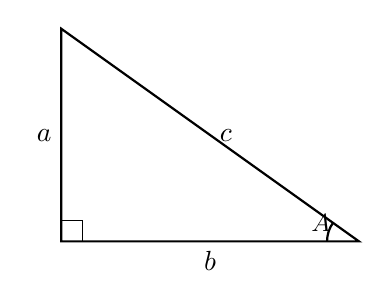
\begin{tikzpicture}[scale=0.9]
  \coordinate (B) at (0,0);
  \coordinate (A) at (4.2,0);
  \coordinate (C) at (0,3);
  \draw[thick] (B) -- (A) -- (C) -- cycle;
  \draw ($(B)+(0.30,0)$) -- ($(B)+(0.30,0.30)$) -- ($(B)+(0,0.30)$);
  \draw[thick] ($(A)+(180:0.45)$) arc[start angle=180, end angle=144.5, radius=0.45];
  \node[anchor=west] at ($(A)+(162:0.85)$) {\small $A$};
  \path (B) -- node[below] {$b$} (A);
  \path (A) -- node[right] {$c$} (C);
  \path (B) -- node[left]  {$a$} (C);
\end{tikzpicture}
\qquad
$\cos(A) = \dfrac{b}{c} \qquad
 \sin(A) = \dfrac{a}{c} \qquad
 \tan(A) = \dfrac{a}{b}$
\end{center}

\begin{regelbox}
\textbf{Regel:} Pythagoras siger $a^{2} + b^{2} = c^{2}$. Skal du finde en
katete, isolerer du først --- så kvadratroden til sidst.
\end{regelbox}

\textbf{Eksempel: trekant med $b = 12$, $c = 13$. Find $a$.}
\begin{align*}
  a^{2} + b^{2} &= c^{2}\\
  a^{2}         &= c^{2} - b^{2}\\
  a^{2}         &= 13^{2} - 12^{2} = 169 - 144 = 25\\
  a             &= \sqrt{25} = 5
\end{align*}
Tjek: $\cos(A) = \tfrac{12}{13}$, $\sin(A) = \tfrac{5}{13}$, $\tan(A) = \tfrac{5}{12}$.

% ── Opgave 2.1 ──────────────────────────────────────────────────────────────
\subsection*{Opgave 2.1 --- Find hypotenusen}

\noindent
I en retvinklet trekant er de to kateter $7\,\text{cm}$ og $24\,\text{cm}$.
Find hypotenusen $c$.

\begin{center}
\trek{24}{7}{$A$}{$b=24\,\text{cm}$}{$c$}{$a=7\,\text{cm}$}{0.32}
\end{center}

\begin{flushright}
\begin{minipage}{0.55\textwidth}
\small\textbf{Tip:} $c = \sqrt{a^{2}+b^{2}} = \sqrt{7^{2}+24^{2}}
= \sqrt{49+576} = \sqrt{625} = 25\,\text{cm}$.
\end{minipage}
\end{flushright}

% ── Opgave 2.2 ──────────────────────────────────────────────────────────────
\subsection*{Opgave 2.2 --- Find den manglende katete}

\noindent
Hypotenusen er $c = 17\,\text{cm}$. Den hosliggende katete ($b$) til vinklen
er $8\,\text{cm}$. Find den modstående katete ($a$).

\begin{center}
\trek{8}{15}{$A$}{$b=8\,\text{cm}$}{$c=17\,\text{cm}$}{$a=?$}{0.55}
\end{center}

\begin{flushright}
\begin{minipage}{0.55\textwidth}
\small\textbf{Tip:} $a = \sqrt{c^{2}-b^{2}} = \sqrt{17^{2}-8^{2}}
= \sqrt{289-64} = \sqrt{225} = 15\,\text{cm}$.
\end{minipage}
\end{flushright}

% ── Opgave 2.3 ──────────────────────────────────────────────────────────────
\subsection*{Opgave 2.3 --- Brug $\sin$, $\cos$ og $\tan$}

\noindent
I trekanten er $a = 6\,\text{cm}$ (modstående), $b = 8\,\text{cm}$
(hosliggende), $c = 10\,\text{cm}$ (hypotenuse).

\begin{center}
\trek{8}{6}{$A$}{$b=8\,\text{cm}$}{$c=10\,\text{cm}$}{$a=6\,\text{cm}$}{0.4}
\end{center}

\noindent
Beregn vinklen $A$ --- og bekræft dit svar ved at tjekke alle tre
trigonometriske forhold.

\begin{flushright}
\begin{minipage}{0.6\textwidth}
\small\textbf{Tip:} $\sin(A) = a/c = 6/10 = 3/5$, så
$A = \sin^{-1}(3/5) \approx 36{,}87^{\circ}$.
Tjek: $\sin^{2}A + \cos^{2}A = (3/5)^{2} + (4/5)^{2} = 9/25+16/25 = 1$.
\end{minipage}
\end{flushright}

% ═════════════════════════════════════════════════════════════════════════════
\newpage
\section{Brøk-regneregler}
% ═════════════════════════════════════════════════════════════════════════════

\subsection*{Regel 1 --- Forlæng og forkort}

\begin{regelbox}
\textbf{Regel:} Forlæng: gang tæller og nævner med det samme tal. Forkort:
divider tæller og nævner med det samme tal. Brøken har samme værdi.
\end{regelbox}

\textbf{Eksempel: Forlæng $\tfrac{2}{7}$ med $5$, forkort $\tfrac{12}{18}$.}
\begin{align*}
  \text{Forlæng:} \quad \frac{2}{7} &= \frac{2\cdot 5}{7\cdot 5} = \frac{10}{35}\\[4pt]
  \text{Forkort:} \quad \frac{12}{18} &= \frac{12\div 6}{18\div 6} = \frac{2}{3}
\end{align*}

\begin{opgavebox}
\textbf{Opgave 3.1} \quad Forlæng $\tfrac{3}{8}$ med $4$. Hvad bliver det?
\end{opgavebox}

\begin{opgavebox}
\textbf{Opgave 3.2} \quad Forkort $\tfrac{24}{32}$ så meget som muligt.
\end{opgavebox}

\subsection*{Regel 2 --- Brøk plus/minus brøk (forskellig nævner)}

\begin{regelbox}
\textbf{Regel:} Find en fællesnævner (et tal som begge nævnere går op i).
Forlæng derefter begge brøker, så de har samme nævner. Så kan du lægge
tællerne sammen.
\end{regelbox}

\textbf{Eksempel: $\tfrac{2}{5} + \tfrac{1}{3}$.}
\begin{align*}
  \text{Fællesnævner for $5$ og $3$ er $15$.}\\
  \frac{2}{5} &= \frac{6}{15}, \qquad \frac{1}{3} = \frac{5}{15}\\[4pt]
  \frac{6}{15} + \frac{5}{15} &= \frac{11}{15}
\end{align*}

\begin{opgavebox}
\textbf{Opgave 3.3} \quad Regn $\tfrac{2}{5} + \tfrac{1}{3}$ --- vis hvordan
du finder fællesnævneren.
\end{opgavebox}

\begin{opgavebox}
\textbf{Opgave 3.4} \quad Regn $\tfrac{5}{7} - \tfrac{2}{3}$
\end{opgavebox}

\subsection*{Regel 3 --- Brøk plus/minus heltal}

\begin{regelbox}
\textbf{Regel:} Skriv heltallet som en brøk med nævner $1$ (fx
$4 = \tfrac{4}{1}$), og brug derefter Regel 2.
\end{regelbox}

\textbf{Eksempel: $\tfrac{3}{8} + 4$.}
\begin{align*}
  \frac{3}{8} + \frac{4}{1} &= \frac{3}{8} + \frac{32}{8}\\[2pt]
  &= \frac{35}{8}
\end{align*}

\begin{opgavebox}
\textbf{Opgave 3.5} \quad Regn $\tfrac{3}{8} + 4$
\end{opgavebox}

\begin{opgavebox}
\textbf{Opgave 3.6} \quad Regn $\tfrac{7}{9} - 5$
\end{opgavebox}

\subsection*{Regel 4 --- Gange brøker}

\begin{regelbox}
\textbf{Regel:} Gang tæller med tæller, nævner med nævner. Forkort til
sidst hvis du kan. $\dfrac{a}{b}\cdot\dfrac{c}{d} = \dfrac{ac}{bd}$.
\end{regelbox}

\textbf{Eksempel: $\tfrac{3}{8}\cdot\tfrac{2}{5}$.}
\[
  \frac{3}{8}\cdot\frac{2}{5} = \frac{3\cdot 2}{8\cdot 5} = \frac{6}{40} = \frac{3}{20}
\]

\begin{opgavebox}
\textbf{Opgave 3.7} \quad Regn $\tfrac{4}{9}\cdot\tfrac{3}{5}$
\end{opgavebox}

\subsection*{Regel 5 --- Dividere brøker}

\begin{regelbox}
\textbf{Regel:} At dividere med en brøk er det samme som at gange med den
omvendte brøk. $\dfrac{a}{b}\div\dfrac{c}{d} = \dfrac{a}{b}\cdot\dfrac{d}{c}$.
\end{regelbox}

\textbf{Eksempel: $\tfrac{5}{9}\div\tfrac{4}{7}$.}
\[
  \frac{5}{9}\div\frac{4}{7} = \frac{5}{9}\cdot\frac{7}{4} = \frac{35}{36}
\]

\begin{opgavebox}
\textbf{Opgave 3.8} \quad Regn $\tfrac{5}{9}\div\tfrac{4}{7}$
\end{opgavebox}

% ═════════════════════════════════════════════════════════════════════════════
\newpage
\section{Regnearter --- udfyld de tomme bokse}
% ═════════════════════════════════════════════════════════════════════════════

\noindent
I de følgende udtryk står $a$ og $b$ for tal, der er større end $0$. Du skal
indsætte et af de fire regnetegn ($+$, $-$, $\cdot$, $\div$) i hver boks, så
udtrykket er korrekt for \emph{alle} værdier af $a$ og $b$. Du må gerne
bruge samme regnetegn i flere bokse, men du må \emph{ikke} bruge parenteser.

\begin{regelbox}
\textbf{Regel:} Gange ($\cdot$) og dividere ($\div$) binder stærkere end
plus ($+$) og minus ($-$). Så $a + b \cdot c$ betyder $a + (b\cdot c)$.
Tip: Tjek altid dit svar med konkrete værdier (fx $a=2$ og $b=3$) --- så
ved du med det samme, om ligheden holder for alle $a, b > 0$.
\end{regelbox}

\textbf{Eksempel:} Løs $a \ \regnebox\ a \ \regnebox\ b \ \regnebox\ b = b^{2}$.
\textbf{Løsning:} Sæt minus, plus og gange i:
$a \;[-]\; a \;[+]\; b \;[\cdot]\; b \;=\; a - a + b\cdot b \;=\; 0 + b^{2} = b^{2}$.
Udregn $b \cdot b$ først (gange binder stærkere), så står der $a - a + b^{2}$.

\subsection*{Opgave 4.1 --- Find de tre regnetegn}

\noindent
Indsæt de tre regnetegn ($+$, $-$, $\cdot$, $\div$) i hvert udtryk, så
ligningen holder for alle $a, b > 0$.

\vspace{6pt}
\begin{center}
\renewcommand{\arraystretch}{2.0}
\begin{tabular}{rcl}
$1)$ & $a \ \regnebox\ a \ \regnebox\ b \ \regnebox\ b \ =\ a^{2} - b^{2}$ & \\[6pt]
$2)$ & $a \ \regnebox\ a \ \regnebox\ b \ \regnebox\ b \ =\ 0$             & \\[6pt]
$3)$ & $a \ \regnebox\ a \ \regnebox\ b \ \regnebox\ b \ =\ a^{2} + b^{2}$ & \\[6pt]
$4)$ & $a \ \regnebox\ a \ \regnebox\ b \ \regnebox\ b \ =\ b^{2} + 1$     & \\[6pt]
$5)$ & $a \ \regnebox\ a \ \regnebox\ b \ \regnebox\ b \ =\ 2b$            & \\[6pt]
$6)$ & $a \ \regnebox\ a \ \regnebox\ b \ \regnebox\ b \ =\ 2$             & \\
\end{tabular}
\end{center}

\begin{flushright}
\begin{minipage}{0.7\textwidth}
\small\textbf{Tip:} Tjek med $a=2$ og $b=3$ for hvert udtryk. Hvis
ligheden holder for netop de to værdier, og du ikke har brugt parenteser,
så holder den for alle $a, b > 0$.
\end{minipage}
\end{flushright}

% ═════════════════════════════════════════════════════════════════════════════
\newpage
\section*{Appendix --- Facit}

\noindent\textbf{Ligninger}
\begin{itemize}[leftmargin=2em, itemsep=2pt]
  \item \textbf{1.1:} $4x+9=33 \Rightarrow 4x=24 \Rightarrow x=6$
  \item \textbf{1.2:} $6x-11=13 \Rightarrow 6x=24 \Rightarrow x=4$
  \item \textbf{1.3:} $7x-5=2x+30 \Rightarrow 5x=35 \Rightarrow x=7$
  \item \textbf{1.4:} $4x-7=x+14 \Rightarrow 3x=21 \Rightarrow x=7$
  \item \textbf{1.5:} $5(x+1)-6=4x+8 \Rightarrow 5x-1=4x+8 \Rightarrow x=9$
  \item \textbf{1.6:} $3(x-4)+7=2x+11 \Rightarrow 3x-5=2x+11 \Rightarrow x=16$
  \item \textbf{1.7:} $3(x+2)-2(x-5)=28 \Rightarrow x+16=28 \Rightarrow x=12$
  \item \textbf{1.8:} $5(2x-3)-3(x+4)=8 \Rightarrow 7x-27=8 \Rightarrow x=5$
\end{itemize}

\noindent\textbf{Trigonometri}
\begin{itemize}[leftmargin=2em, itemsep=2pt]
  \item \textbf{2.1:} $c^{2}=7^{2}+24^{2}=49+576=625 \Rightarrow c=\sqrt{625}=25\,\text{cm}$
  \item \textbf{2.2:} $a^{2}=c^{2}-b^{2}=17^{2}-8^{2}=289-64=225 \Rightarrow a=15\,\text{cm}$
  \item \textbf{2.3:} $\sin A = \tfrac{6}{10}=\tfrac{3}{5}$, $\cos A = \tfrac{4}{5}$, $\tan A = \tfrac{3}{4}$; $A = \sin^{-1}(3/5) \approx 36{,}87^{\circ}$; tjek: $(3/5)^{2}+(4/5)^{2} = 9/25+16/25 = 1$ \checkmark
\end{itemize}

\noindent\textbf{Brøk-regneregler}
\begin{itemize}[leftmargin=2em, itemsep=2pt]
  \item \textbf{3.1:} $\tfrac{3}{8} = \tfrac{12}{32}$
  \item \textbf{3.2:} $\tfrac{24}{32} = \tfrac{3}{4}$
  \item \textbf{3.3:} Fællesnævner $15$: $\tfrac{6}{15}+\tfrac{5}{15} = \tfrac{11}{15}$
  \item \textbf{3.4:} Fællesnævner $21$: $\tfrac{15}{21}-\tfrac{14}{21} = \tfrac{1}{21}$
  \item \textbf{3.5:} $\tfrac{3}{8}+\tfrac{4}{1} = \tfrac{3}{8}+\tfrac{32}{8} = \tfrac{35}{8}$
  \item \textbf{3.6:} $\tfrac{7}{9}-\tfrac{5}{1} = \tfrac{7}{9}-\tfrac{45}{9} = -\tfrac{38}{9}$
  \item \textbf{3.7:} $\tfrac{4}{9}\cdot\tfrac{3}{5} = \tfrac{12}{45} = \tfrac{4}{15}$
  \item \textbf{3.8:} $\tfrac{5}{9}\cdot\tfrac{7}{4} = \tfrac{35}{36}$
\end{itemize}

\noindent\textbf{Regnearter (Opgave 4.1)}
\begin{itemize}[leftmargin=2em, itemsep=2pt]
  \item \textbf{4.1.1)} $a \;\mathbf{\cdot}\; a \;\mathbf{-}\; b \;\mathbf{\cdot}\; b \;=\; a^{2} - b^{2}$ \ \ (tjek $a=2,b=3$: $4-9=-5 = 2^{2}-3^{2}$ \checkmark)
  \item \textbf{4.1.2)} $a \;\mathbf{-}\; a \;\mathbf{+}\; b \;\mathbf{-}\; b \;=\; 0$ \ \ (tjek: $2-2+3-3=0$ \checkmark)
  \item \textbf{4.1.3)} $a \;\mathbf{\cdot}\; a \;\mathbf{+}\; b \;\mathbf{\cdot}\; b \;=\; a^{2} + b^{2}$ \ \ (tjek: $4+9=13 = 2^{2}+3^{2}$ \checkmark)
  \item \textbf{4.1.4)} $a \;\mathbf{\div}\; a \;\mathbf{+}\; b \;\mathbf{\cdot}\; b \;=\; 1 + b^{2}$ \ \ (tjek: $1+9=10 = 3^{2}+1$ \checkmark)
  \item \textbf{4.1.5)} $a \;\mathbf{\div}\; a \;\mathbf{\cdot}\; b \;\mathbf{+}\; b \;=\; b + b = 2b$ \ \ (tjek: $3+3=6 = 2\cdot 3$ \checkmark)
  \item \textbf{4.1.6)} $a \;\mathbf{\div}\; a \;\mathbf{+}\; b \;\mathbf{\div}\; b \;=\; 1 + 1 = 2$ \ \ (tjek: $1+1=2$ \checkmark)
\end{itemize}

\end{document}
